\chapter{Fundamentos teóricos}
    \section{TRNGs}
    \section{Jitter}
    \section{Pruebas estadísticas}
    \section{Mapas caóticos}


    \section{Teoría de FPGAs en Xilinx}
        Para poder realizar la implementación del núcleo ERO es necesario utilizar las primitivas y macros propias del fabricante de FPGA que para este trabajo es Xilinx. Las primitivas son componentes de Xilinx que son nativos de la arquitectura a la que se dirige y los macros son elementos que se encuentran en las bibliotecas UniMacro y Xilinx Parameterized Macros, las cuales se utilizan para instanciar elementos que son complejos de instanciar simplemente usando las primitivas, después las herramientas de síntesis expanden automáticamente estas macros a sus primitivas subyacentes. Los métodos de diseño disponibles son la instanciación, la inferencia, el catalogo IP y el soporte de macros, no obstante para este diseño solo se utilizan la instanciación, la cual permite instanciar un componente directamente en el diseño y es útil si se desea controlar el uso, la implementación y la ubicación exactos de los bloques individuales y el soporte de macros, el cual, utilizando las librerías antes mencionadas permiten abstraer la complejidad de utilizar unicamente primitivas simples.

        Toda la información referente a los macros y primitivas se encuentran en la documentación oficial en el archivo llamado ``Vivado Design Suite 7 Series FPGA Libraries Guide''. Para poder utilizar las primitivas y las macros es necesario agregar la librería UniMacro en la cabecera del archivo VHDL de la siguiente manera: 

        \vspace{0.4cm}
        \lstinputlisting[style = VHDL_TEXT, caption = Librería para primitivas de Xilix., label = cod:library]{codigos/vhdl_codes/primitivas/library.vhd}
        % \lstinputlisting[style = VHDL_TEXT]{codigos/vhdl_codes/primitivas/library.vhd}

	    \subsection{Primitivas}

		    \subsubsection{LUT1: 1-Bit Look-Up Table with General Output}
	
                \begin{figure}[hbtp]
                    \caption{Esquemático de LUT1.}
                    \centering
                    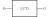
\includegraphics[width=0.3\linewidth]{D2_lut1}
                    \label{fig:D2_lut1}
                \end{figure}	
	
                Este elemento proporciona una versión de look-up table de un búfer o inversor. Estos elementos son los bloques de construcción básicos. El parámetro INIT le da a la LUT su valor lógico. De forma predeterminada, este valor es cero, lo que lleva la salida a cero independientemente de los valores de entrada (actuando como tierra).Sin embargo, en la mayoría de los casos hay que determinar un nuevo valor INIT para especificar la función lógica de la primitiva LUT. Existen al menos dos métodos mediante los cuales se puede determinar el valor LUT. El método de la tabla lógica y el método de ecuación. En la Tabla \ref{tab:lut1} se muestran las entradas y salidas y la forma de configurar INIT y en el Código \ref{cod:lut1} se muestra su implementación en VHDL.

                \begin{table}[htbp]
                    \centering
                    \caption{Tabla lógica de LUT1.}
                    \begin{tabular}{|cc|}
                        \hline
                        \multicolumn{1}{|c|}{\textbf{Inputs}} & \textbf{Outputs} \\ 
                        \multicolumn{1}{|c|}{\textbf{I0}} & \textbf{O} \\ 
                        \hline 
                        \multicolumn{1}{|c|}{0} & INIT[0] \\ \hline
                        \multicolumn{1}{|c|}{1} & INIT[1] \\ \hline
                        \multicolumn{2}{|c|}{INIT = Binary number assigned to the INIT attribute} \\ 
                        \hline
                    \end{tabular}
                    \label{tab:lut1}
                \end{table}	
	
                \vspace{0.4cm}
                \lstinputlisting[style = VHDL_TEXT, caption = Primitava de LUT1., label = cod:lut1]{codigos/vhdl_codes/primitivas/lut1.vhd}
                % \lstinputlisting[style = VHDL_TEXT]{codigos/vhdl_codes/primitivas/lut1.vhd}

            \subsubsection{OBUFDS: Differential Signaling Output Buffer}

                \begin{figure}[hbtp]
                    \caption{Esquemático de OBUFDS.}
                    \centering
                    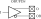
\includegraphics[width=0.3\linewidth]{D3_obufds}
                    \label{fig:D3_obufds}
                \end{figure}	

                Este elemento de diseño es un búfer de salida única que admite señalización diferencial de bajo voltaje. OBUFDS aísla el circuito interno y proporciona corriente de accionamiento para las señales que salen del chip. Su salida se representa como dos puertos distintos (O y OB), uno considerado el ``maestro'' y el otro el ``esclavo''. El maestro y el esclavo son fases opuestas de la misma señal lógica.  En la Tabla \ref{tab:obufds} se muestran las entradas y salidas y en el Código \ref{cod:obufds} se muestra su implementación en VHDL.
                
                \begin{table}[htbp]
                    \centering
                    \caption{Tabla lógica de OBUFDS.}
                    \begin{tabular}{|c|cc|}
                        \hline
                        \textbf{Inputs} & \multicolumn{2}{c|}{\textbf{Outputs}} \\ 
                        \textbf{I}      & \multicolumn{1}{c}{\textbf{O}}  & \textbf{OB} \\ 
                        \hline
                        0      & \multicolumn{1}{c|}{0}  & 1  \\ \hline
                        1      & \multicolumn{1}{c|}{1}  & 0  \\ \hline
                    \end{tabular}
                    \label{tab:obufds}
                \end{table}

                \vspace{0.4cm}
                \lstinputlisting[style = VHDL_TEXT, caption = Primitava de OBUFDS., label = cod:obufds]{codigos/vhdl_codes/primitivas/obufds.vhd}
                % \lstinputlisting[style = VHDL_TEXT]{codigos/vhdl_codes/primitivas/obufds.vhd}
\begin{comment}

Datos para programar la tarjeta

Default Board: Basys3
Default Part: xc7a35tcpg236-1
Product: Artix-7
Family: Artix-7
Package: cpg236
Speed Grade: -1

\end{comment}

    
    %\section{Selección y evaluación de núcleos TRNGs}

%-----------------------------------------------------------------

	Los números aleatorios se utilizan en muchos ámbitos de nuestra vida. Los utilizamos para elegir quién gana la lotería, decidir la dirección en la que atacará un equipo en el primer tiempo de un partido de futbol, asegurar una partida limpia en un juego de mesa y desempeñan un papel fundamental en la criptografía y la seguridad de la información. Para seleccionar qué equipo decide el lado del campo basta con lanzar una moneda. Para jugar a un juego de mesa, necesitamos más de dos valores aleatorios, por lo que utilizamos un dado. La criptografía, en cambio, requiere algo más que tirar un dado para asegurar nuestros datos en comunicaciones digitales o en transacciones bancarias. La seguridad de las comunicaciones es una parte muy importante de la vida moderna. En esta era de la información, la gente envía correos electrónicos, llama o envía mensajes a sus amigos y realiza transacciones en línea millones de veces al día. Se supone que cada uno de estos procesos cotidianos es seguro y confidencial. La seguridad de la comunicación depende de la capacidad de estos procesos para verificar que las personas que se comunican son realmente quienes dicen ser. La seguridad sólo puede lograrse mediante la distribución de identidades privadas conocidas sólo por el usuario individual, conocidas como claves, de modo que personas maliciosas no puedan suplantar a nadie y causar algún tipo de daño. Una clave privada es un gran número generado aleatoriamente que es único para el usuario. La aleatoriedad de los números de las claves privadas determina la seguridad de las conexiones. La capacidad de generar números aleatorios es, por tanto, una parte muy importante de la seguridad de los sistemas de comunicación.

	En un sistema criptográfico, los generadores de números aleatorios o Random Number Generators (RNG) por sus siglas en inglés se utilizan no sólo para generar claves criptográficas, sino también para generar nonces, valores de relleno, vectores de inicialización, desafíos y máscaras aleatorias para la protección contra ataques de canal lateral \cite{Petura2016}. A pesar de que hay muchas aplicaciones diferentes de los números aleatorios, todos comparten dos requisitos básicos: buenas propiedades estadísticas, concretamente una distribución de probabilidad uniforme, cada valor de cualquier número aleatorio debe tener la misma probabilidad de aparecer e imprevisibilidad de los números aleatorios. Los números aleatorios, especialmente los utilizados para parámetros secretos como las claves, deben ser impredecibles para evitar que un atacante pueda calcular valores futuros o anteriores a partir de los datos ya generados y capturados. En los diseños modernos, se requieren algunas características adicionales: el generador debe ser intrínsecamente seguro, robusto y resistente a los ataques y probado en línea mediante pruebas específicas del generador \cite{Badrignans2011}.
		
	Dado el amplio rango de aplicaciones de los RNG, existan diferentes clases de RNG que satisfacen diversas necesidades. Basándonos en el método utilizado para generar números aleatorios, hay dos tipos fundamentales de RNG:
		
	\begin{enumerate}
		\item Generadores de números aleatorios deterministias (DRNG/PRNG)
		
		También conocidos como generadores de números pseudo-aleatorios (PRNG), son sistemas que producen una secuencia de aspecto aleatorio de forma matemática, hay un algoritmo subyacente y debido a esto los DRNG son fáciles de implementar en dispositivos lógicos \cite{Jun1999}. Si se conoce el algoritmo, la salida del generador es predecible. Incluso cuando no se conoce el algoritmo pero se han guardado algunas de las secuencias de salida del generador, su comportamiento durante la secuencia guardada puede utilizarse en futuros ataques. Los números producidos parecen aleatorios a corto plazo, pero la secuencia es periódica, normalmente con un periodo largo. Para producir una salida menos predecible, estos generadores utilizan valores de inicialización llamados semillas para empezar \cite{Nist2010}. Para cada semilla se genera una secuencia diferente. Por esta razón, los DRNG deben ser computacionalmente seguros, el algoritmo no debe poder adivinarse computacionalmente y su valor inicial nunca debe reutilizarse. La reutilización del valor inicial puede evitarse guardando el último valor haciendo uso de un contador y utilizando el siguiente valor del contador la próxima vez. La secuencia de salida de un buen DRNG está perfectamente distribuida de manera uniforme, tienen buenas propiedades estadísticas. Los DRNGs consiguen altas tasas de bits de salida y suelen utilizarse como generadores de claves en los cifrados de flujo \cite{Badrignans2011}.
		
		\item Generadores de números aleatorios verdaderos (TRNG)
		
		Son sistemas que extraen la aleatoriedad de fenómenos aleatorios no algorítmicos. Estos fenómenos pueden ser fluctuaciones de temperatura, decaimiento radiactivo, ruido de radio ambiental, tiempos de acceso al disco duro o interacciones del usuario con el PC. Dado que los fenómenos utilizados son intrínsecamente impredecibles, los TRNG producen datos aleatorios reales en lugar de simples secuencias periódicas de aspecto aleatorio. El comportamiento de un TRNG no está definido por una fórmula matemática, como es el caso de los DRNG. Dado que la calidad de la secuencia aleatoria generada depende de las propiedades físicas, la secuencia de salida puede presentar algunos defectos estadísticos, como el 	sesgo. Las características estadísticas de los TRNG suelen ser peores que las de los DRNG	y están estrechamente relacionadas con la calidad de la fuente de entropía, pero también con el método de extracción de la aleatoriedad. La velocidad final de los TRNG está limitada por el espectro de la señal aleatoria y por el principio utilizado para extraer la entropía de la misma por ejemplo, la frecuencia de muestreo vinculada al espectro del ruido. Los TRNG son, en general, más lentos que los DRNG. En función de la fuente utilizada, pueden dividirse en:
		\begin{itemize}
			\item Físicos (PTRNG), utiliza ruido físico a nivel de electrones presente en todos los semiconductores. Es un dispositivo físico y utiliza ruido físico.
			\item No físicos (NPTRNG, puede no ser un dispositivo físico, sino una pieza de software. Utiliza una fuente de aleatoriedad no física, como las interacciones del usuario con un sistema operativo.
		\end{itemize}
	\end{enumerate}
	
	La imprevisibilidad de los generadores de números aleatorios deterministas está garantizada computacionalmente, mientras que la imprevisibilidad de los generadores verdaderamente aleatorios está garantizada por fenómenos físicos aleatorios y se caracteriza por la tasa de entropía a la salida del generador. Tanto los TRNG como los DRNG tienen sus ventajas y desventajas, por lo que muchos sistemas criptográficos utilizan RNG híbridos. Los generadores de números aleatorios híbridos (HRNG) representan una combinación de un RNG determinista (rápido y de buena calidad) sembrado repetidamente por un RNG físico (lento pero impredecible). Se debe encontrar un compromiso entre la velocidad del generador y su previsibilidad ajustando el intervalo de tiempo entre semillas y el tamaño de una semilla. 	En función de su implementación, existen dos tipos de RNGs híbridos:
	
	\begin{enumerate}
		\item Generadores de números aleatorios verdaderos híbridos
		
		Combinan un TRNG con un postprocesamiento criptográfico. El postprocesamiento criptográfico asegura el secreto hacia adelante y hacia atrás de los números aleatorios producidos, no pueden calcularse los valores pasados o los futuros a partir del valor actual. Si la fuente física falla, también garantiza unas propiedades estadísticas perfectas de los datos de salida, ya que el núcleo de un postprocesamiento criptográfico suele ser un cifrador. La tasa de bits de salida de un TRNG híbrido está limitada por la del núcleo del TRNG.
		
		\item Generadores de números aleatorios deterministas híbridos. 
		
		Utilizan un TRNG para generar periódicamente semillas para un DRNG. Dado que la salida de un DRNG es predecible si conocemos su semilla, ir renovando la semilla mediante un TRNG puede reducir la predictibilidad de un DRNG híbrido. La secuencia de salida de un generador de este tipo es perfectamente uniforme, lo que podría no ser el caso de un TRNG puro. Su tasa de bits de salida viene determinada por la tasa de bits del DRNG subyacente, ya que se pueden producir números aleatorios mientras no se alcance el periodo de repetición del DRNG.
	\end{enumerate}
		
	A pesar de la menor velocidad de los TRNG, estos se utilizan con más frecuencia en aplicaciones criptográficas que los DRNG. Los TRNG son las únicas primitivas criptográficas que no han sido objeto de normalización hasta ahora. Sin embargo, antes de utilizar un generador en la práctica, el principio de funcionamiento y su implementación dentro de un módulo criptográfico deben ser validados por una institución acreditada como parte de un proceso de evaluación de seguridad. Los generadores que no tienen un certificado de seguridad se consideran inseguros en cuanto a su uso en aplicaciones criptográficas. Por este motivo, es de gran interés el estudio de los principales TRNG existentes.
	
	Para evitar que los atacantes accedan a las claves confidenciales, éstas deben generarse dentro del sistema criptográfico. Dado que los sistemas criptográficos actuales implementan esencialmente algoritmos y protocolos criptográficos, en su mayoría se implementan en dispositivos lógicos y sistemas digitales. Por lo tanto, es natural orientar la investigación hacia la implementación de generadores de números aleatorios en dispositivos lógicos, concretamente en matrices de puertas programables en campo (FPGA).
	
	\section{Estructura de los TRNG}	
		
	La estructura general de un TRNG se muestra en la Figura \ref{fig:A1_TRNG_estructura}. El generador debe utilizar un proceso físico incontrolable como fuente de aleatoriedad. Dado que los fenómenos físicos utilizados en los TRNG son en su mayoría procesos analógicos, suele ser necesario algún método que permita la conversión de datos del dominio analógico al digital. Se puede incluir una conversión de analógico a digital en el procedimiento de extracción de aleatoriedad. La señal binaria sin procesar obtenida, el llamado ruido digital, puede tener baja entropía, malas propiedades estadísticas o ambas. En este caso, se pueden usar algunos algoritmos de post-procesamiento para mejorar los parámetros estadísticos del flujo de bits de salida. Sin embargo, el post-procesamiento de la salida del TRNG a veces puede enmascarar una falla grave en el generador. Las pruebas estadísticas estándar pueden entonces fallar en detectar la debilidad enmascarada. Por lo tanto, se recomienda tener la posibilidad de probar el ruido digital sin procesar (RBS). La seguridad del generador se puede aumentar si las pruebas estadísticas se aplican sobre la marcha y si están diseñadas para adaptarse al principio de funcionamiento del generador teniendo presente sus posibles debilidades.
			
	\begin{figure}[hbtp]
		\caption{Estructura general de un TRNG \cite{Badrignans2011}.}
		\centering
		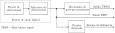
\includegraphics[width=0.9\textwidth]{A0_TRNG_estructura}
		\label{fig:A1_TRNG_estructura}
	\end{figure}
	
	Los TRNG usan diferentes fuentes de aleatoriedad y numerosos principios para extraerla. Se utilizan tres clases de características para evaluar a los TRNG: parámetros relacionados con la calidad, con la seguridad y con el diseño.
			
	\begin{itemize}[noitemsep]
		\item Parámetros relacionados con la calidad
			\begin{itemize}[noitemsep]
				\item Fuente de aleatoriedad
				\item Método de extracción de aleatoriedad y entropía del ruido digital
				\item Método de procesamiento posterior aplicado (opcional)
				\item Tasa de bits de salida y su estabilidad
			\end{itemize}
		\item Parámetros relacionados con la seguridad
			\begin{itemize}[noitemsep]
				\item Existencia de un modelo matemático
				\item Comprobabilidad interna
				\item Seguridad (robustez, resistencia contra ataques)
			\end{itemize}
		\item Parámetros relacionados con el diseño
			\begin{itemize}[noitemsep]
				\item El uso de recursos
				\item El consumo de energía
				\item Viabilidad en dispositivos lógicos y FPGAs
				\item Automatización del diseño
			\end{itemize}
	\end{itemize}
			
	Es importante señalar que estas características de los TRNG no son todas igualmente importantes. Los parámetros de seguridad como la robustez, la disponibilidad de un modelo estocástico, la capacidad de prueba, etc. siempre tienen prioridad en un sistema de seguridad de datos. Su peso en la evaluación de TRNG es mucho mayor que el de otros parámetros como el consumo de energía, la tasa de bits, etc \cite{Badrignans2011}.
			
	\section{Parámetros relacionados con la calidad}	
	
		\subsection{Fuentes de aleatoriedad en dispositivos lógicos}
	
	
	Los TRNG pueden utilizar fuentes de ruido físicas o no físicas. En los dispositivos lógicos, las fuentes de ruido físico son bastante limitadas, ya que en teoría los dispositivos lógicos están siempre en un estado bien definido, están diseñados para la implementación de sistemas lógicos deterministas. Para generar números aleatorios, necesitamos un fenómeno aleatorio incontrolable. Los fenómenos físicos más utilizados para generar números aleatorios en los dispositivos lógicos son:
	
	\begin{itemize}[noitemsep]
		\item Metastabilidad: es la capacidad de un circuito de persistir en un estado indefinido durante un periodo de tiempo indefinido.
		
		\item Variación del reloj (Clock jitter): es una variación del flanco del reloj desde su posición ideal.
		
		\item Caos: es un comportamiento imprevisible de un sistema determinista, muy sensible a sus condiciones iniciales.
		
		\item Señales analógicas: como el ruido de disparo de un diodo, el ruido térmico, etc.		
	\end{itemize}		
	
	Cualquier comportamiento imprevisible en un sistema de este tipo puede tener consecuencias catastróficas para el comportamiento del sistema global. Aunque los eventos impredecibles debidos a la naturaleza física de la tecnología son inevitables, los vendedores de dispositivos lógicos tienden a minimizarlos. Por esta razón, los métodos de extracción de aleatoriedad utilizados en el diseño del TRNG deben ser examinados críticamente para mantenerse al día con la evolución de la tecnología. La mayoría de los dispositivos lógicos, y concretamente los FPGA, no contienen bloques analógicos y de tenerlos seria necesario un convertidor analógico-digital para poder utilizar una señal analógica, lo cual agrega otra capa de complejidad. Por esta razón las fuentes de aleatoriedad más utilizadas en dispositivos lógicos están relacionadas con el funcionamiento de las puertas lógicas. Se pueden utilizar varios fenómenos y sus combinaciones: la variación del retardo de las puertas lógicas, el comportamiento analógico de las puertas lógicas entre dos niveles lógicos (la metaestabilidad), la violación del tiempo de preparación y retención y el ruido térmico generado dentro del dispositivo.	
					
	La inestabilidad de los retardos de las puertas lógicas provoca variaciones en la propagación de la señal a lo largo del tiempo. Estas variaciones pueden verse como una inestabilidad del período del reloj (jitter) en los generadores de reloj que contienen elementos de retardo ensamblados en un circuito cerrado (osciladores en anillo).
					
	Dado que las resistencias y los condensadores se pueden implementar fácilmente en la tecnología digital, el ruido térmico generado en las resistencias se puede utilizar para modular la frecuencia de un oscilador de funcionamiento libre (oscilador RC). El ruido térmico se convierte así al dominio del tiempo, donde se puede extraer fácilmente. Sin embargo, este principio no se puede utilizar en FPGA, porque no se dispone de estructuras apropiadas.
					
	Algunos generadores utilizan el jitter de seguimiento introducido por los bucles de bloqueo de fase, phase locked loops (PLL), para generar números aleatorios. Los PLLs analógicos son fáciles de implementar en dispositivos digitales, incluyendo los FPGA, porque el filtro RC que está en tales PLLs, es en su mayoría el único bloque ``analógico'', puede ser fácilmente implementado usando la misma tecnología. Por lo tanto, se puede considerar un TRNG basado en PLL como un generador que puede implementarse en dispositivos lógicos en general.
	
	
	\subsection{Métodos de extracción de aleatoriedad}	
	
	En los dispositivos lógicos que no contienen un bloque analógico, la aleatoriedad a menudo se extrae mediante el muestreo de una señal de reloj en los flancos ascendentes o descendentes de una señal de reloj de referencia utilizando flip-flops síncronos o asíncronos (latches). El flujo de bits aleatorio se puede obtener de dos formas: muestreando señales aleatorias a intervalos regulares o muestreando señales regulares a intervalos de tiempo aleatorios. En sistemas síncronos, el primer método es preferible para garantizar una tasa de bits constante en la salida.
					
	La elección entre flip-flops síncronos y asíncronos es importante en los FPGA. Esto se debe a que los flip-flops síncronos están cableados en celdas lógicas como bloques optimizados y, en consecuencia, su comportamiento metaestable se minimiza. Por otro lado, los latches generalmente solo se pueden implementar en Look-Up Tables  y, por lo tanto, están sujetos a un comportamiento metaestable en mayor medida. 
	
	%Hasta el momento, el comportamiento de flip-flops síncronos y asíncronos y su uso para la extracción de aleatoriedad en FPGAs no ha sido suficientemente evaluado. 
					
	El método de extracción de aleatoriedad suele estar vinculado al principio básico del generador y a la fuente de aleatoriedad. El procedimiento de extracción de aleatoriedad y el post-procesamiento a veces se fusionan en el mismo bloque y no se pueden separar. En ese caso, la entropía de la fuente de aleatoriedad se modifica mediante el post-procesamiento y no se puede medir ni evaluar correctamente. 
					
	En el proceso de evaluación de los TRNG, la fuente de aleatoriedad y el método de extracción de aleatoriedad están estrechamente vinculados y no se pueden separar. Por esta razón, es más razonable evaluar estos dos parámetros del generador juntos. La mejor forma de hacerlo es evaluando la entropía incluida en el ruido digital.
		
	\subsection{Técnicas de post-procesamiento}
					
		La evaluación de los TRNG casi siempre se basa en pruebas estadísticas que se aplican a secuencias aleatorias producidas por el TRNG. A veces, la fuente de entropía puede tener algunas debilidades que conducen a la producción de números no aleatorios, secuencias largas de ceros o unos. Por esta razón, el post-procesamiento puede ser necesario para mejorar las propiedades estadísticas de los números aleatorios, por ejemplo, para aumentar la entropía por bit, reducir el sesgo y la correlación. 
					
	La calidad de la señal de ruido digital, la señal obtenida en el bloque de extracción de aleatoriedad, puede deteriorarse por varias razones: 
	
	\begin{enumerate}[noitemsep, label=(\alph*)]
		\item La entropía de la fuente no es lo suficientemente alta, este suele ser el caso si se utiliza la metaestabilidad como fuente de aleatoriedad.
		\item La entropía, que es alta en la señal original, no está bien extraída
		\item Las muestras extraídas están correlacionadas. La entropía por bit a la salida del generador aumenta principalmente a costa de la reducción y/o variación de la tasa de bits.
	\end{enumerate}		
	
	
	El objetivo del bloque de post-procesamiento es hacer que la secuencia de salida no se distinga de la secuencia aleatoria ideal, que no está correlacionada y tiene una distribución uniforme. Existen dos tipos principales de post-procesamiento:
	
	\begin{enumerate}
		\item Post-procesamiento algorítmico
		
		Utiliza algún algoritmo de procesamiento de datos para mejorar los parámetros estadísticos de los números generados. Puede tratarse de la XOR de varios bits de salida, la corrección de Von Neumann, varios tipos de algoritmos de compresión, etc.
		
		\item Posprocesamiento criptográfico 
		
		Utiliza algún algoritmo criptográfico seguro para asegurar la imprevisibilidad de los números generados en dirección hacia adelante y/o hacia atrás si la fuente física de aleatoriedad falla. El uso de un post-procesamiento criptográfico mejora la solidez del TRNG frente a los ataques.
	\end{enumerate}
		
	Las técnicas más utilizadas para el post-procesamiento de la señal obtenida en el bloque de extracción de aleatoriedad son: 
	
	\begin{itemize}
		\item Corrector XOR 
		
		Es una función lineal simple que aplica una operación OR exclusiva en bloques no superpuestos de $n$ bits para generar un bit de salida. Puede reducir drásticamente el sesgo de la salida del generador a costa de reducir su tasa de bits $n$ veces. Sin embargo, el sesgo del flujo de bits de salida sólo se reduce si los bits originales son independientes. Las principales ventajas del corrector XOR son su simplicidad y la posibilidad de mantener una tasa de bits de salida constante.

		\item Corrector de Von Neumann
		
		Es una sencilla función no lineal que toma pares de bits sucesivos y, si los bits no son iguales, utiliza el primer bit del par y descarta los pares idénticos. Por tanto, la tasa de bits de salida depende de los datos. 
		
		Aunque el flujo de entrada es estacionario y puede estar sesgado, la salida será insesgada. Sin embargo, si el flujo original está autocorrelacionado, la salida puede seguir estando autocorrelacionada. También el corrector producirá una salida sesgada si el flujo de entrada presenta un ciclo con periodo 2. Si el corrector se implementa en hardware, puede interferir con el generador y provocar exactamente este tipo de ocurrencia.
		
		
		\item Registros de desplazamiento de retroalimentación lineal (LFSRs)
		
		Linear Feedback Shift Registers en inglés, se utilizan en muchos generadores de flujos de bits aleatorios. Hay varias razones para ello, son fáciles de implementar en hardware, pueden producir secuencias de gran periodo, pueden producir secuencias con buenas propiedades estadísticas y  debido a su estructura, pueden ser fácilmente analizados utilizando técnicas algebraicas.	Un LFSR de longitud $L$ consta de $L$ elementos de retardo, cada uno de los cuales puede almacenar un bit y tiene una entrada y una salida, y un reloj que controla el movimiento de los datos. Durante cada unidad de tiempo, se realizan las siguientes operaciones:
		\begin{enumerate}[noitemsep, label=(\roman*)]
			 \item El contenido del primer elemento de retardo sale y forma parte de la secuencia de salida.
			 \item  El contenido del elemento $i$ se mueve a la etapa $i - 1$ para cada $i$, $1 \leq i \leq L - 1$.
			 \item El nuevo contenido del último elemento de retardo es el bit de retroalimentación que se calcula sumando módulo 2 los contenidos anteriores de un subconjunto fijo de elementos, dependiendo del polinomio subyacente.
		 \end{enumerate}	
		
		\item Funciones resilientes
		
		Son funciones específicas utilizadas en criptografía y teoría de la codificación. Derivan de las funciones booleanas. El estudio de las funciones booleanas es muy importante en criptografía, sobre todo en el diseño de algoritmos de clave simétrica.  En términos más informales, las funciones resilientes son adecuadas para el post-procesamiento porque el conocimiento de cualquier $m$ valores de entrada a la función no permite a nadie hacer una conjetura mejor que el azar en la salida. Las funciones resistentes se basan en el mismo principio que los códigos de corrección de errores. Mientras que los códigos de corrección de errores se utilizan para suprimir los errores aleatorios, las funciones resistentes se utilizan para extraer estos bits aleatorios. La señal binaria sin procesar, ruido digital, puede considerarse como un flujo de bits que contiene una redundancia y la función resistente reduce la tasa de bits mientras extrae los bits aleatorios. De este modo, la función resistente aumenta la entropía por bit en la salida del generador.
			
		\item Cifrado de la señal de ruido digital
		
		Este tipo de post-procesamiento del ruido digital utiliza las propiedades de difusión y confusión de las funciones criptográficas. Las características estadísticas perfectas de la mayoría de los algoritmos de cifrado pueden utilizarse para enmascarar las imperfecciones del generador. Una de las ventajas de este enfoque es que la clave de cifrado puede utilizarse como variable criptográfica para modificar dinámicamente el comportamiento del generador. Aunque este tipo de bloque de posprocesamiento, el cifrador, es bastante complejo y caro, el TRNG puede reutilizar (compartir) el cifrador que se utiliza para la codificación de los datos.	
		
		
		\item Hashing de la señal de ruido digital
		
		Uno de los métodos que más tiempo consume, pero también uno de los más seguros, es el post-procesamiento criptográfico basado en funciones hash como MD5, SHA-1 u otras. Utiliza las propiedades de difusión y unidireccionalidad, a diferencia de la codificación de la señal binaria sin procesar, de las funciones hash para garantizar la no previsibilidad de los bits generados por el TRNG si se produce una ruptura total de la fuente de ruido. En este caso, debido a la propiedad de no linealidad de las funciones hash, el TRNG se comportará como un PRNG.
	\end{itemize}
	
	El post-procesamiento puede mejorar la tasa de entropía a la salida del generador a costa de reducir la tasa de bits de salida, sin embargo nunca puede generar entropía.
	El objetivo es producir números aleatorios en sin procesar de alta calidad para que no sea necesario el post-procesamiento. Este enfoque es especialmente útil en aplicaciones de alta seguridad.
		
	\subsection{Tasa de bits de salida}
	
	La velocidad es un parámetro secundario considerando la seguridad en muchas aplicaciones criptográficas. Las velocidades de bits de salida van desde 100kbps  hasta 1Mbps. Sin embargo, hay algunas aplicaciones de seguridad de datos de velocidad crítica para las que se requieren generadores de alta velocidad. Los servidores de telecomunicaciones de alta velocidad son un segundo ejemplo. Necesitan generar claves de sesión de forma regular a alta velocidad, decenas de megabits por segundo. Un servidor Ethernet de 10 Gbit necesitaría alrededor de 20 Mbps de bits aleatorios para generar una clave de sesión de 128 bits para cada bloque de datos de 64 kB para poder resistir los ataques de canal lateral. 
					
	Otro aspecto de la tasa de bits de salida que debe tenerse en cuenta es su variabilidad. Algunos generadores dan números aleatorios periódicamente, otros generan resultados en intervalos de tiempo irregulares. En el segundo caso, se requiere un registro para acumular los números generados. Otra solución es estimar la tasa de bits más pequeña disponible en la salida y muestrear la salida a esta tasa. La desventaja de la primera solución es que, según la tasa de bits de salida media y la necesidad de números aleatorios, los registros a veces deben ser muy grandes. La desventaja de la segunda solución es que si la tasa de bits estimada es incorrecta, los números aleatorios a veces pueden no estar disponibles en la salida.	
	
	
	\section{Parámetros relacionados con la seguridad}
	
	\subsection{Modelado matemático de TRNG}
	
	La parte principal de un proceso de certificación de seguridad se ocupa de la evaluación del diseño y la implementación del generador. El objetivo de la evaluación es cuantificar la entropía por bit aleatorio. Sin embargo, la entropía es una propiedad de variables aleatorias y no de realizaciones observadas. Para cuantificar la entropía, necesitamos analizar la distribución de las variables aleatorias, por ejemplo mediante el uso de un modelo estocástico. El modelo estocástico especifica una familia de distribuciones de probabilidad de variables aleatorias que permite verificar un límite de entropía inferior para la señal binaria sin procesar. El valor dado por el modelo se puede utilizar para probar la entropía de los números generados en tiempo real
				
	\subsection{Comprobabilidad}
	
	
	La comprobabilidad interna significa que la estructura del generador permite evaluar la entropía de la señal sin procesar, esta debe estar disponible. Esta funcionalidad es necesaria en los procedimientos de evaluación recientes de TRNG. Sin embargo, cuando la extracción de la aleatoriedad y el post-procesamiento se fusionan en el mismo proceso, la señal aleatoria sin procesar no está disponible. Incluso cuando esta señal está disponible, a veces está compuesta por un patrón pseudoaleatorio combinado con un flujo de bits verdaderamente aleatorio. El patrón pseudoaleatorio dificulta la evaluación estadística de la señal.
				

				
	\subsection{Evaluación de seguridad}
				
	A menudo es muy difícil y a veces imposible construir un modelo estocástico para un generador en particular. En ese caso, se puede utilizar otro enfoque para validar el uso del generador en aplicaciones criptográficas. Este enfoque se basa en el análisis del impacto del entorno cambiante o un ataque al generador. Hay tres posibilidades: 
	
	\begin{enumerate}[noitemsep, label=(\roman*)]
		\item Existe prueba de que el generador no puede funcionar mal como resultado de un ataque o de un entorno cambiante.
		\item No existe prueba de seguridad ni ataque.
		\item Se ha informado de algún ataque a un generador en particular.
	\end{enumerate}		

	\section{Parámetros relacionados con el diseño}	
		
	\subsection{Uso de recursos}
				
	Para evaluar varios principios de TRNG, es importante analizar los recursos necesarios para la implementación del hardware del generador. En términos generales, todo tipo de recursos disponibles en FPGA se pueden utilizar para generar números aleatorios: celdas lógicas basadas en LUT o basadas en multiplexor, bloques de memoria integrados, bloques de reloj con PLL y DLL, osciladores RC integrados, multiplicadores cableados, interconexiones programables, etc.
					
	Los FPGA tienen muchas celdas lógicas, por lo que el uso de celdas lógicas  no suele ser un problema. La topología y los parámetros eléctricos de las interconexiones programables dependen en gran medida de la tecnología. Muchos diseños de TRNG requieren la intervención manual del diseñador durante la colocación y el enrutamiento. Algunos diseños pueden implementarse fácilmente en una familia de FPGA, pero son difíciles o imposibles de implementar en otras. La elección y el número de bloques cableados integrados suele ser mucho más limitado y varía según el proveedor y la tecnología. Por lo tanto, el uso de bloques cableados puede ser un factor limitante para la reutilización del principio TRNG.
				
	\subsection{Consumo de energía}
					
	El consumo de energía del generador está vinculado a su fuente de aleatoriedad, a la frecuencia de reloj utilizada y a la agilidad del algoritmo. En aplicaciones de energía crítica, el generador se puede detener cuando no está en uso. Sin embargo, la posibilidad de controlar la generación de flujo de bits se puede utilizar para atacar al generador.
					
	\subsection{Viabilidad en FPGAs}
				
	En comparación con la implementación de TRNG en ASIC, su implementación en FPGA es mucho más restrictiva. Muchos TRNG implementados en ASIC utilizan componentes analógicos para generar aleatoriedad y para procesar la aleatoriedad, como amplificadores operacionales o comparadores. La mayoría de estos bloques generalmente no están disponibles en FPGA, aunque algunos de ellos pueden estar disponibles en familias seleccionadas, como PLL analógicos en la mayoría de las familias Altera, pero no en todas las familias de Xilinx. Algunos generadores no son viables o son difíciles de implementar, algunos otros son viables en FPGAs seleccionados pero los principios más generales son factibles en todas las FPGAs.
				
	\subsection{Automatización del diseño}
				
	El hecho de que el generador utilice recursos que están disponibles en FPGAs no significa automáticamente que pueda ser implementado en este tipo de dispositivos. El rango de tolerancia de algunos parámetros tecnológicos puede ser tal que impida la implementación confiable del generador. El parámetro que más suele limitar la implementación del generador en FPGA es la disponibilidad de los recursos de enrutamiento y sus características. Algunos generadores requieren un enrutamiento perfectamente equilibrado. Esto requiere un control perfecto de la ubicación del módulo, por ejemplo, ubicación simétrica de dos módulos en relación con otro módulo y enrutamiento. Si bien la mayoría de las herramientas de diseño de FPGA permiten un control preciso de la ubicación, el proceso de enrutamiento es difícil o imposible de controlar. Incluso cuando el enrutamiento se puede controlar parcial o totalmente en las familias Altera y Xilinx, los retrasos en la red de enrutamiento configurable varían tanto de un dispositivo a otro que es imposible equilibrar las interconexiones de los módulos de manera general y el diseño dependerá del dispositivo, es decir, debe equilibrarse manualmente para cada dispositivo. Tal intervención manual no es aceptable desde el punto de vista de la implementación práctica del generador. Los mejores generadores se pueden mapear automáticamente, sin intervención manual en todas las familias de FPGA. Desde el punto de vista práctico, sigue siendo aceptable si la implementación del generador requiere intervención manual para cada familia o tipo de dispositivo. Sin embargo, los generadores que requieren optimización manual por dispositivo no son aceptables para aplicaciones industriales.
	
	
	\section{Evaluación de los TRNG}
	
		\subsection{Condiciones de funcionamiento y calidad de la salida del TRNG}
	
	La salida de un buen TRNG debe ser indistinguible de la salida de un TRNG ideal, independientemente de las condiciones de funcionamiento y del tiempo. La calidad del flujo de bits de salida del generador y sus parámetros de seguridad, incluyendo la robustez frente al envejecimiento, los cambios ambientales, los ataques, la existencia de autopruebas y las pruebas en línea, son muy importantes en el diseño del TRNG. Los buenos TRNGs dan un flujo de ceros y unos uniformemente distribuido a su salida. La calidad de la salida del generador está estrechamente ligada a la calidad de la fuente de aleatoriedad y al método de extracción de aleatoriedad utilizado. Las características de la fuente de aleatoriedad y de la extracción de aleatoriedad determinan los principales parámetros del flujo de bits generado: el sesgo del flujo de bits de salida, la correlación entre los bits posteriores, los patrones visibles, etc. Aunque algunos de estos fallos pueden corregirse mediante un post-procesamiento eficaz, es mejor que el generador produzca intrínsecamente un flujo de bits sin procesar de buena calidad.
	
	Si el extractor muestrea la fuente de aleatoriedad demasiado rápido, los bits adyacentes podrían estar correlacionados. Por esta razón, es una buena práctica comprobar el flujo de bits generado para detectar una autocorrelación a corto plazo. También es posible que el ruido digital presente otras dependencias a corto plazo, que deben ser detectadas por algunas pruebas específicas del generador. El comportamiento del generador suele estar influenciado por interferencias eléctricas externas e internas. El efecto más evidente serán las frecuencias discretas procedentes de la fuente de alimentación y de diversas señales internas que aparecen en el espectro de ruido. El espectro de la señal de ruido generada puede estar significativamente influenciado por un ruido de baja frecuencia causado por los semiconductores. Además, las frecuencias altas del espectro de ruido pueden ser filtradas involuntariamente por algunas capacidades internas.

	Algunos generadores pueden presentar los llamados puntos malos. Los puntos malos son períodos cortos en los que el generador deja de funcionar, posiblemente debido a interferencias eléctricas o externas de la parte sobrecargada del circuito del generador. Otra característica peligrosa del generador puede ser una puerta trasera, que se refiere a las desviaciones de la aleatoriedad uniforme introducidas deliberadamente por el fabricante. Por ejemplo, supongamos que en lugar de utilizar algún proceso físico, el generador generara una secuencia pseudoaleatoria de alta calidad con una semilla de 40 bits. Sería imposible detectar este comportamiento aplicando pruebas estadísticas estándar en el flujo de bits de salida, pero sería computacionalmente factible para alguien que conozca la puerta trasera adivinar las claves sucesivas.
	
	
		\subsection{Estándares para el diseño y certificación de TRNG}
	
	Diferentes aplicaciones criptográficas requieren distintos niveles de seguridad, por lo que es necesario estandarizar el uso de la criptografía para aplicaciones específicas. Ya existen muchos estándares que proporcionan algoritmos estándar para el cifrado como el AES, RSA o funciones hash como la SHA-3. Pero debido a la naturaleza de los TRNG, que son específicos de la tecnología y de la plataforma, no hay forma de proporcionar un diseño estandarizado. Por ello, varias autoridades de certificación han desarrollado diferentes enfoques estándar para la certificación de TRNG.
	
	El primer intento de certificación del diseño del TRNG requería únicamente probar las propiedades estadísticas de los números generados. Se propusieron muchos conjuntos de pruebas para conseguirlo, como FIPS 140-1 [Agragar ref], DIEHARD [Agregar ref], NIST 800-22 [Agregar ref], entre otras. La idea de las pruebas estadísticas de los TRNG es que un TRNG debe producir una secuencia de salida que no se distinga de la ideal. Una secuencia aleatoria ideal es estacionaria, se distribuye uniformemente y sus muestras son independientes. De hecho, las propiedades estadísticas de los números generados pueden comprobarse fácilmente mediante pruebas estadísticas adecuadas, pero no su independencia. El problema con este tipo de pruebas de TRNG es que trata a un TRNG como una caja negra y sólo considera su salida. Ahora bien, si colocamos un buen generador de números pseudoaleatorios en lugar de un TRNG, su salida pasará todo tipo de pruebas estadísticas. Esto se debe a que los buenos generadores de números pseudoaleatorios están hechos de algoritmos que producen secuencias con propiedades estadísticas perfectas. Sin embargo, su resultado no es realmente aleatorio, sólo parece serlo. Al final son algoritmos y como tales, su comportamiento está claramente definido y es predecible.
	
	La evaluación de las propiedades estadísticas de un TRNG es necesaria, pero claramente no es suficiente. Por ello, existen normas más recientes que exigen la caracterización de la fuente de ruido además de las pruebas estadísticas. Estas normas son la AIS-20/31, elaborada por la Oficina Federal de Seguridad de la Información de Alemania, (BSI) por sus siglas en Alemán [Agregar ref], y la NIST 800-90B, del Instituto Nacional de Normas y Tecnología de Estados Unidos [Agregar ref]. Aunque las dos normas utilizan una metodología de evaluación ligeramente diferente, ambas comparten la misma idea básica de una arquitectura TRNG. La Figura \ref{fig:A1_TRNG_estructura} muestra el diagrama de bloques de un TRNG tal y como lo especifican tanto AIS-20/31 como NIST 800-90B.
	
	La fuente de ruido digital está compuesta por una fuente de ruido analógica y un digitalizador. Este bloque produce el ruido digital, al que nos referimos como señal binaria sin procesar. También es el único bloque que extrae la verdadera aleatoriedad del proceso subyacente, por lo que es el único que genera la entropía. Su salida debe estar disponible para su evaluación, con el fin de comprobar la calidad de la señal sin procesar y estimar la tasa de entropía en la salida. El bloque de post-procesamiento es un proceso algorítmico y, por lo tanto, podemos calcular fácilmente la tasa de entropía a su salida, que también es la salida del generador, a partir de la tasa de entropía a su entrada, que se conoce a partir del modelo y que puede verificarse probando los datos de la señal sin procesar. Según la norma AIS-20/31, el post-procesamiento no debe reducir la entropía. Ambas normas consideran el post-procesamiento, como una opción. Lo ideal sería que un buen TRNG no requiriera ningún tipo de post-procesamiento algorítmico.
	
	Las pruebas integradas son la tercera parte necesaria del diseño del TRNG. Según la AIS- 20/31, estas pruebas contienen al menos dos tipos de pruebas: la prueba de fallo total y las pruebas en línea. La prueba de fallo total debe informar muy rápidamente de la pérdida completa de entropía en la fuente con una baja probabilidad de falsas alarmas. Dicha pérdida total de la fuente de entropía podría ser un cambio rápido o la pérdida total de la conexión física con la fuente. Las pruebas en línea, por otro lado, deben ser capaces de detectar defectos irreparables intolerables en la secuencia de salida. El defecto irreparable es un fallo estadístico que no puede ser corregido por el post-procesamiento. Este defecto puede producirse cuando el dispositivo funciona fuera de su rango de parámetros de funcionamiento, por ejemplo, por una sobre o baja tensión, temperaturas extremas, o algún otro fenómeno inesperado. Las pruebas en línea pueden ejecutarse de forma continua, a petición, o activarse por un evento interno específico. Sin embargo, las pruebas tienen que pasar con éxito cada vez que el TRNG se inicie o reinicie, funcionando efectivamente también como pruebas de encendido.

		\subsection{Resumen de los requisitos del AIS-20/31 sobre los TRNG}
	
	La norma AIS-20/31 reconoce varias clases diferentes de TRNGs en función de su principio de funcionamiento:
	
	\begin{itemize}[noitemsep]
		\item Tres clases PTG para los generadores de números aleatorios verdaderos físicos (PTRNG), clases PTG.1 a PTG.3.
		\item Cuatro clases de DRG para los generadores aleatorios deterministas (DRNG), clases DRG.1 a DRG.4.
		\item Una clase NTG para los generadores de números aleatorios verdaderos no físicos, (NPTRNG), clase NTG.1.
	\end{itemize}
	
	Dado que nos estamos centrando en los TRNG físicos, vamos a echar un vistazo a las clases PTG.
	
	Todas las clases de TRNG deben superar las pruebas estadísticas de caja negra. Estas pruebas se dividen en dos procedimientos de prueba descritos en la norma AIS-20/31:
	
	\begin{itemize}[noitemsep]
		\item El procedimiento de prueba A contiene las pruebas estadísticas T0 a T5. Estas pruebas verifican las propiedades estadísticas generales, como el sesgo, y están destinadas a comprobar los datos post-procesados.
		
		\item El procedimiento de prueba B contiene las pruebas T6 a T8. Las pruebas T6 y T7 detectan la dependencia entre los números generados. La prueba T8 compara la entropía de Shannon estimada por bit con un umbral de 0.997. El procedimiento de prueba B está destinado a comprobar los datos sin procesar.
	\end{itemize}		
	Tanto los identificadores como el nombre de la prueba son los siguientes:
	\begin{itemize}[noitemsep]
		\item T0: Prueba de disyunción
		\item T1: Prueba de monobit 
		\item T2: Prueba de póquer
		\item T3: Prueba de corridas
		\item T4: Prueba de corridas larga
		\item T5: Prueba de auto-correlación
		\item T6: Prueba de distribución uniforme
		\item T7: Prueba de homogeneidad
		\item T8: Estimación de la entropía
	\end{itemize}
	
	\subsubsection{Clase PTG1 TRNG}
		PTG.1 es una clase de TRNG físico de baja seguridad destinado a aplicaciones que no son críticas para la seguridad. La figura 1.18 muestra el diagrama de bloques de dicho generador y los puntos de prueba requeridos por la norma.
		
		\paragraph{Requisitos de la fuente de aleatoriedad\\}
		
		No se requiere ningún modelo estocástico para un PTG.1 TRNG. Sin embargo, la fuente de ruido debe ser física, estar claramente definida y descrita para que quede claro el origen de la aleatoriedad.
		
		\paragraph{Pruebas integradas\\}
		
		La clase PTG.1 requiere la implementación de pruebas de fallo total y en línea. La prueba de fallo total debe detectar un fallo completo de la fuente de aleatoriedad. Las pruebas en línea deben supervisar continuamente y garantizar la calidad estadística de los números aleatorios producidos. La clase PTG.1 requiere que las pruebas en línea supervisen la calidad de los números aleatorios internos (es decir, a la salida del generador).
		
		\paragraph{Post-procesamiento\\}
		
		La clase PTG.1 no requiere que el TRNG utilice ningún tipo de posprocesamiento. Tampoco desaconseja el uso del posprocesamiento. Sin embargo, un TRNG PTG.1 debe superar las pruebas estadísticas del Procedimiento de prueba A, por lo que el posprocesamiento puede ser necesario si la señal binaria bruta no puede superar dichas pruebas
		
	\subsubsection{Clase PTG2 TRNG}
	
		PTG.2 es una clase de TRNG físico, que puede utilizarse para generar claves criptográficas, nonces, semillas para DRNGs, etc. En comparación con la clase PTG.1 de baja seguridad, el TRNG PTG.2 debe garantizar el secreto de los números aleatorios producidos (su imprevisibilidad). La figura 1.19 muestra la estructura interna y las pruebas necesarias para el TRNG PTG.2.
	
		\paragraph{Requisitos de la fuente de aleatoriedad\\}
		
			Todos los requisitos de la clase PTG.1 se aplican también a la clase PTG.2. Además, se requiere un modelo estocástico para la fuente de aleatoriedad. El modelo estocástico debe tener en cuenta el comportamiento de la fuente de aleatoriedad. Basándose en los parámetros de la fuente, el modelo estima la entropía de la señal binaria bruta. La entropía de Shannon de la señal binaria bruta debe ser superior a 0,997 por bit según la norma AIS-20/31.
		
		
		\paragraph{Pruebas integradas\\}
		
			Para un TRNG PTG.2 es necesario implementar tanto las pruebas de fallo total como las pruebas en línea. La prueba de fallo total debe detectar un fallo de la fuente de aleatoriedad total.

			 Las pruebas en línea deben detectar las debilidades estadísticas intolerables de la señal binaria bruta. Deben funcionar con una señal binaria sin procesar porque el uso del posprocesamiento podría enmascarar algunos defectos potencialmente peligrosos. Las pruebas en línea deben adaptarse al modelo estocástico. De este modo, pueden detectar los defectos específicos de la fuente de aleatoriedad utilizada de forma muy eficaz.

		\paragraph{Post-procesamiento\\}
		
			De forma similar a la clase PTG.1, la clase PTG.2 no requiere el posprocesamiento cuando la señal binaria bruta proporciona números aleatorios de suficiente calidad. Si el post-procesamiento es necesario, la clase PTG.2 no pone ninguna restricción en el algoritmo utilizado, sin embargo, no debe reducir la entropía.
		
	
	\subsubsection{Clase PTG3 TRNG}
	
		PTG.3 es una clase TRNG híbrida para TRNGs de alta seguridad. Los TRNG de esta clase no se basan únicamente en la seguridad proporcionada por la fuente de aleatoriedad, sino que añaden una segunda ancla de seguridad en forma de post-procesamiento criptográficamente seguro. Un TRNG híbrido es un TRNG compuesto por un TRNG físico, que vuelve a alimentar continuamente al TRNG determinista. En este caso, el TRNG determinista sirve como post-procesamiento para el TRNG físico que genera entropía. La figura 1.20 muestra el diagrama de bloques de un TRNG híbrido de este tipo.
	
	\paragraph{Requisitos de la fuente de aleatoriedad\\}
	
		La fuente de aleatoriedad del TRNG PTG.3 debe cumplir todos los requisitos de la clase PTG.2. La entropía de Shannon de la señal binaria bruta debe ser superior a 0,997 por bit, lo que debe estar garantizado por el modelo estocástico de la fuente.
	\paragraph{Pruebas integradas\\}
	
		Además de las pruebas de fallo total y en línea que se exigen también para el TRNG PTG.2, la clase PTG.3 requiere también la prueba de respuesta conocida (KAT) para el posprocesamiento. Esta prueba debe pasar con éxito cada vez que se inicie/reinicie el TRNG para verificar el correcto funcionamiento del algoritmo de posprocesamiento.
		
	\paragraph{Post-procesamiento\\}
	
	A diferencia de los requisitos de PTG.1 y PTG.2, la clase PTG.3 requiere el uso de un post-procesamiento (criptográfico). Además, requiere el uso de un DRNG de la clase DRG.3, que proporciona secreto hacia delante y hacia atrás mejorado. Esto significa, efectivamente, que el post-procesamiento para un TRNG de clase PTG.3 debe ser una función criptográfica. Una mayor discusión sobre el tema de los DRNG está fuera del alcance de esta tesis y remitimos al lector interesado a [25].
	
		\subsection{Resumen de los requisitos del NIST 800-90B sobre los TRNG}
	
		El NIST 800-90B exige, al igual que el AIS-20/31, que la secuencia de salida del TRNG pase las pruebas de caja negra. Estas pruebas de caja negra se dividen en dos vías:
		
		\begin{itemize}[noitemsep]
			\item La pista IID se utiliza para datos independientes e idénticamente distribuidos (IID)
			\item La pista no IID se utiliza para los datos que no superan la prueba de detección de IID. Además de superar las pruebas de caja negra, el NIST 800-90B también impone requisitos a los bloques individuales del TRNG.
		\end{itemize}
		
		\paragraph{Fuente de ruido\\}
		
			El NIST 800-90B tiene los siguientes requisitos sobre la fuente de ruido:
			
		\begin{itemize}[noitemsep]
			\item Hay que describir su comportamiento.
			\item Su salida debe ser estacionaria.
			\item Debe indicarse la entropía de salida esperada.
			\item Debe protegerse de la observación e influencia de los adversarios.
			\item La fuente de ruido debe tener un comportamiento aleatorio.
		\end{itemize}
		
		Aunque la norma exige la declaración de estacionariedad de la salida y de entropía esperada, no requiere ninguna prueba matemática de estas afirmaciones. Sólo es necesaria la descripción técnica de por qué se cree que la fuente de ruido tiene el comportamiento afirmado.
		
		
		\paragraph{Pruebas de salud\\}
		
		El NIST 800-90B exige tres tipos de pruebas de salud.
		
		\begin{itemize}[noitemsep]
			\item Las pruebas de puesta en marcha deben verificar si todos los componentes necesarios de la fuente de ruido funcionan correctamente. La fuente de ruido no debe emitir datos antes de que las pruebas de puesta en marcha se completen con éxito.
			\item Las pruebas continuas comprueban los defectos y fallos en el comportamiento de la fuente de ruido. Estas pruebas se realizan de forma continua en todas las muestras emitidas por la fuente de ruido. El NIST 800-90B exige que se utilicen dos pruebas continuas aprobadas. Además de las pruebas aprobadas, también se pueden utilizar pruebas definidas por el desarrollador. La norma permite a los desarrolladores no utilizar las pruebas aprobadas, pero en su lugar deben utilizarse otras pruebas continuas que pueden detectar el mismo tipo de defectos que las pruebas aprobadas.
			\item Las pruebas a la carta no se realizan hasta que se solicitan. Debe haber una forma de realizar pruebas a demanda en la fuente de ruido. Las muestras utilizadas para las pruebas a demanda no deben salir hasta que las pruebas se completen con éxito.
		\end{itemize}
		
		\paragraph{Acondicionamiento\\}
		
		El NIST 800-90B entiende el componente de acondicionamiento como una "función determinista responsable de reducir el sesgo y/o aumentar la tasa de entropía de los bits de salida resultantes" [32]. El componente de acondicionamiento es completamente opcional, por lo que puede omitirse por completo.
		
		La entropía de salida del TRNG se estima después del componente de condicionamiento. El estándar proporciona una lista de algoritmos de condicionamiento comprobados, para los que los desarrolladores pueden reclamar una entropía completa, aunque esta reclamación tiene que ser validada. Estos algoritmos son funciones hash combinadas con cifrado de bloques (para una lista completa, consulte [32]).
		
		Se permite el uso de componentes de acondicionamiento no validados, pero estos componentes son penalizados en términos de estimación de entropía. Cuando se utiliza un componente condicionante no validado, la entropía en la salida se multiplica por una constante de 0,999, lo que le impide alcanzar la entropía completa.
		
		\subsection{Conclusiones de la certificación de seguridad TRNG}
		
		Hay dos normas principales relativas a los TRNG que están en vigor en la actualidad:
		
		\begin{itemize}[noitemsep]
			\item AIS-20/31 utilizado en muchos países europeos. [25]
			\item NIST 800-90B utilizado en los Estados Unidos [32]
		\end{itemize}
	
	Se está preparando una norma internacional con la identificación ISO/IEC PRF 20543, pero no se ha publicado en el momento de escribir esta tesis, ya que todavía está en fase de aprobación.
	
	Las dos normas existentes en la actualidad exigen que el diseño de un TRNG esté bien documentado y su funcionamiento interno bien descrito, además de las pruebas estadísticas. También exigen que se realicen pruebas integradas, de modo que un TRNG se supervise continuamente durante su funcionamiento.
	
	Sin embargo, la norma AIS-20/31 profundiza en el problema de la descripción del TRNG y exige que se desarrolle también un modelo estocástico. Las pruebas integradas, según la AIS-20/31, también deben implementarse de acuerdo con el modelo estocástico. Este requisito no se cumple en la norma NIST 800-90B, que da más libertad en el diseño del TRNG, pero no en sus pruebas implementadas según el modelo estocástico. Este requisito no se cumple en la norma NIST 800-90B, que da más libertad en el diseño del TRNG, pero no en sus pruebas.
	
	En definitiva, AIS-20/31 es más completo y sus requisitos son más estrictos que los de NIST 800-90B. Dado que uno de los objetivos del proyecto HECTOR es proponer diseños de TRNG que cumplan con AIS-20/31, en el resto de la tesis nos centraremos únicamente en los TRNG que cumplan con AIS-20/31. En concreto, nos ocuparemos sólo de los TRNG de clase PTG.2, ya que PTG.1 no necesita un modelo y está destinado a aplicaciones no críticas para la seguridad, y PTG.3 requiere un DRNG, que está fuera del alcance de esta tesis.	

%-----------------------------------------------------------------











	
	\section{Variación del reloj (Clock jitter)}
	
	Se supone que una señal de reloj ideal en los dispositivos lógicos digitales es una señal rectangular con un ciclo de trabajo del 50\% y un periodo estable. Pero debido a los diversos ruidos que afectan a los dispositivos electrónicos, la señal de reloj nunca es absolutamente estable y sus flancos se mueven de su posición estable. En otras palabras, la fase de la señal de reloj fluctúa. Esta fluctuación puede verse como una variación del reloj en el dominio del tiempo y como un ruido de fase en el dominio de la frecuencia. En los dispositivos lógicos, una variación del reloj suele ser indeseado, pero inevitable. Dado que estas variaciones afectan negativamente a las comunicaciones de alta frecuencia y a los sistemas de alta velocidad, ha sido bien estudiado y caracterizado.
	
	En los sistemas analógicos, el jitter se caracteriza mejor en el dominio de la frecuencia. De este modo, los componentes de fase y amplitud pueden estudiarse y caracterizarse por separado. En cambio, en los sistemas digitales, las propiedades temporales del jitter son más importantes y, por tanto, el jitter se caracteriza en el dominio del tiempo.
	
	Las variaciones del reloj en un sistema digital es una desviación del flanco de reloj real con respecto a un flanco de reloj ideal. Una señal de reloj ideal se define mediante la ecuación (\ref{eq:periodic}), donde $t(n)$ representa el tiempo del $n$-ésimo periodo de una señal de reloj y $T$ es el periodo de una señal de reloj.
	
	\begin{equation}
		t(n) =  n T
	\label{eq:periodic}
	\end{equation}
	
	Una señal de reloj real no llega siempre a múltiplos enteros de su periodo, como lo hace la ideal, sino que sus flancos fluctúan en torno a este valor a causa del jitter. El jitter está causado por diversos fenómenos físicos, como el ruido térmico, el ruido de la fuente de alimentación, el ruido electromagnético ambiental, etc.	
	
	
	
	\section{Arquitectura de núcleos TRNG seleccionados}

	Con base en los criterios del AIS-20/31, y los núcleos \gls{TRNG} que usan estructuras oscilantes como se clasifican en \cite{Petura2016}:
	
	\begin{itemize}
		\item Single-event ring oscillators
			\begin{itemize}
				\item Elementary ring oscillator based TRNG (\gls{ERO-TRNG})
				\item Coherent sampling ring oscillator based TRNG (\gls{COSO-TRNG})
				\item Multi-ring oscillator based TRNG (\gls{MURO-TRNG})
			\end{itemize}
		\item Multi-event ring oscillators with signal collisions
			\begin{itemize}
				\item Transient effect ring oscillator based TRNG (\gls{TERO-TRNG})
			\end{itemize}
		\item Multi-event ring oscillators without signal collisions
			\begin{itemize}
				\item Self-timed ring based TRNG (\gls{STR-TRNG})
			\end{itemize}
		\item Phase-locked loops
			\begin{itemize}
				\item PLL based TRNG (\gls{PLL-TRNG})
			\end{itemize}
	\end{itemize}
	
		\subsection{Elementary ring oscillator based TRNG (ERO-TRNG)}
		
					
				\begin{figure}[hbtp]
					\caption{Arquitectura del núcleo ERO-TRNG.}
					\centering
					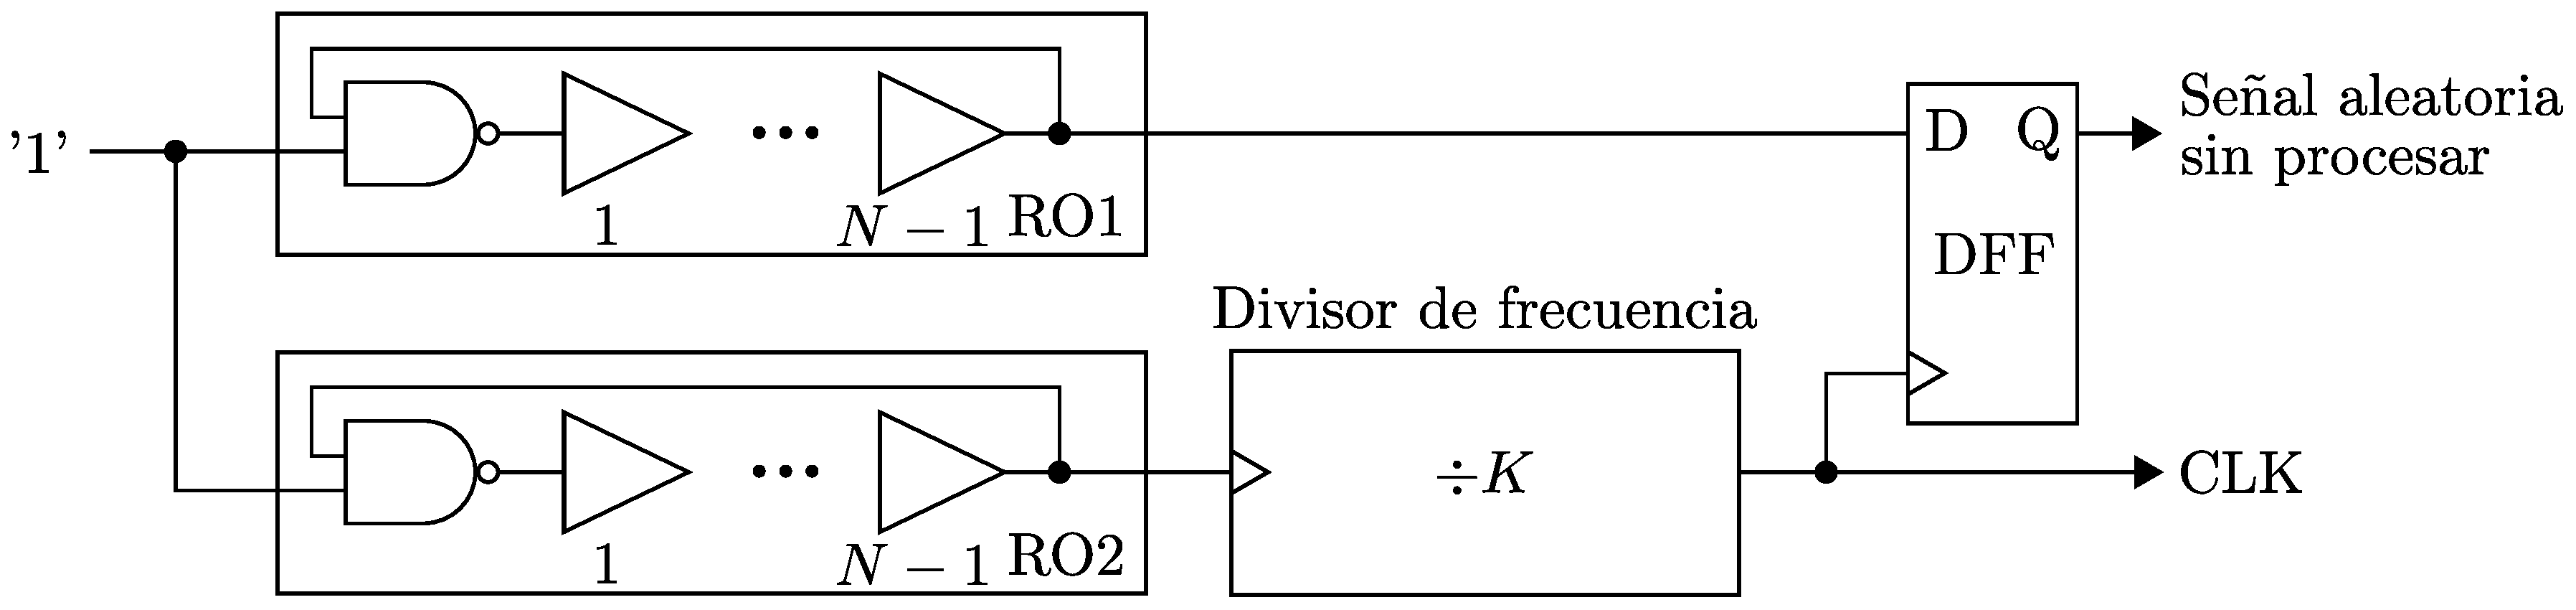
\includegraphics[width=0.8\linewidth]{A1_ERO_TRNG}
					\label{fig:A1_ERO_TRNG}
				\end{figure}
			
			
			
		\subsection{Coherent sampling ring oscillator based TRNG (COSO-TRNG)}
	
				
				\begin{figure}[hbtp]
					\caption{Arquitectura del núcleo COSO-TRNG.}
					\centering
					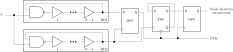
\includegraphics[width=0.8\linewidth]{A2_COSO_TRNG}
					\label{fig:A2_COSO_TRNG}
				\end{figure}
				
				
				
		\subsection{Multi-ring oscillator based TRNG (MURO-TRNG)}
	
				
				\begin{figure}[hbtp]
					\caption{Arquitectura del núcleo MURO-TRNG.}
					\centering
					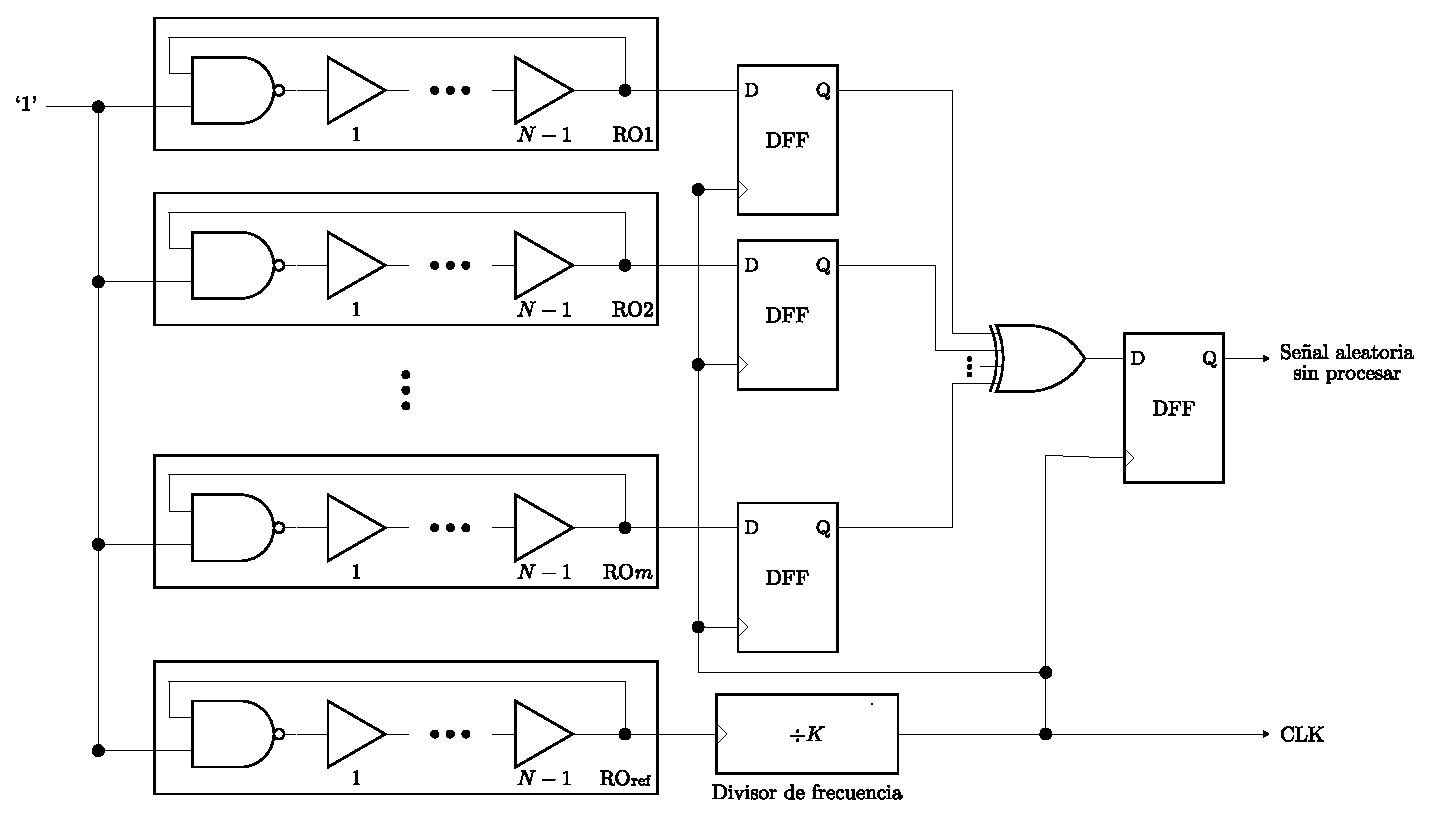
\includegraphics[width=0.8\linewidth]{A3_MURO_TRNG}
					\label{fig:A3_MURO_TRNG}
				\end{figure}
				
				
				
		\subsection{Transient effect ring oscillator based TRNG (TERO-TRNG)}
	
				
				\begin{figure}[hbtp]
					\caption{Arquitectura del núcleo TERO-TRNG.}
					\centering
					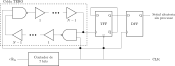
\includegraphics[width=0.8\linewidth]{A4_TERO_TRNG}
					\label{fig:A4_TERO_TRNG}
				\end{figure}
				
				
				
		\subsection{Self-timed ring based TRNG (STR-TRNG)}
	
				
				\begin{figure}[hbtp]
					\caption{Arquitectura del núcleo STR-TRNG.}
					\centering
					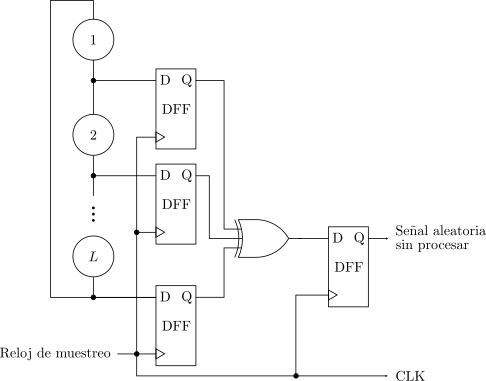
\includegraphics[width=0.8\linewidth]{A5_STR_TRNG}
					\label{fig:A5_STR_TRNG}
				\end{figure}
				
				
				
		\subsection{PLL based TRNG (PLL-TRNG)}
	
				
				\begin{figure}[hbtp]
					\caption{Arquitectura del núcleo PLL-TRNG.}
					\centering
					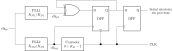
\includegraphics[width=0.8\linewidth]{A6_PLL_TRNG}
					\label{fig:A6_PLL_TRNG}
				\end{figure}
				
				
			
		   



% Table generated by Excel2LaTeX from sheet 'Sheet1'
\begin{table}[htbp]
  \centering
  \caption{Resumen de los resultados de implementación de las TRNGs}
\resizebox{0.8\linewidth}{!}{ 
    \begin{tabular}{|c|c|c|c|c|c|c|c|c|}
    \hline
    \rowcolor[rgb]{ .682,  .667,  .667} TRNG Type & FPGA  & Area  & Power cons. & Bit Rate & Efficiency & Entropy & Entropy * Bit rate & Feasib. \\
    \rowcolor[rgb]{ .682,  .667,  .667}       & device & (LUT/Reg) & [mW]  & [Mbits/s] & [bits/$\mu$Ws] & per bit &       & \& Repeat. \\
    \hline
    \multirow{3}[2]{*}{ERO} & Spartan 6 & 46/19 & 2.16  & 0.0042 & 1.94  & 0.999 & 0.004 & \multirow{3}[2]{*}{5} \\
          & Cyclone V & 34/20 & 3.24  & 0.0027 & 0.83  & 0.990 & 0.003 &  \\
          & SmartFusion 2 & 45/19 & 4     & 0.014 & 3.5   & 0.980 & 0.013 &  \\
    \hline
    \multirow{3}[2]{*}{COSO} & Spartan 6 & 18/3  & 1.22  & 0.54  & 442.6 & 0.999 & 0.539 & \multirow{3}[2]{*}{1} \\
          & Cyclone V & 13/3  & 0.9   & 1.44  & 1600  & 0.999 & 1.438 &  \\
          & SmartFusion 2 & 23/3  & 1.94  & 0.328 & 169   & 0.999 & 0.327 &  \\
    \hline
    \multirow{3}[2]{*}{MURO} & Spartan 6 & 521/131 & 54.72 & 2.57  & 46.9  & 0.999 & 2.567 & \multirow{3}[2]{*}{4} \\
          & Cyclone V & 525/130 & 34.93 & 2.2   & 62.9  & 0.999 & 2.197 &  \\
          & SmartFusion 2 & 545/130 & 66.41 & 3.62  & 54.5  & 0.999 & 3.616 &  \\
    \hline
    \multirow{3}[2]{*}{PLL} & Spartan 6 & 34/14 & 10.6  & 0.44  & 41.5  & 0.981 & 0.431 & \multirow{3}[2]{*}{3} \\
          & Cyclone V & 24/14 & 23    & 0.6   & 43.4  & 0.986 & 0.592 &  \\
          & SmartFusion 2 & 30/15 & 19.7  & 0.37  & 18.7  & 0.921 & 0.340 &  \\
    \hline
    \multirow{3}[2]{*}{TERO} & Spartan 6 & 39/12 & 3.312 & 0.625 & 188.7 & 0.999 & 0.624 & \multirow{3}[2]{*}{1} \\
          & Cyclone V & 46/12 & 9.36  & 1     & 106.8 & 0.987 & 0.985 &  \\
          & SmartFusion 2 & 46/12 & 1.23  & 1     & 813   & 0.999 & 0.999 &  \\
    \hline
    \multirow{3}[2]{*}{STR} & Spartan 6 & 346/256 & 65.9  & 154   & 2343.2 & 0.998 & 154.121 & \multirow{3}[2]{*}{2} \\
          & Cyclone V & 352/256 & 49.4  & 245   & 4959.1 & 0.999 & 244.755 &  \\
          & SmartFusion 2 & 350/256 & 82.52 & 188   & 2286.7 & 0.999 & 188.522 &  \\
    \hline
    \end{tabular}%
}
  \label{tab:addlabel}%

\end{table}%


